\clearpage
\section{Ekonomická vzácnost. Dělení statků. Výrobní faktory a hranice produkčních možností.}

\subsection{Ekonomická vzácnost}
\begin{itemize}
    \item omezenost (aby byl člověk ochoten vynaložit energii na získání nějakého předmětu,
    nesmí být pro něj tento předmět volně dostupný (ne pitná voda z potoku za domem)
    \item užitečnost (daný předmět musí mít pro jedince nějakou užitnou hodnotu (ne lednička
    v~Arktidě)
\end{itemize}

\subsection{Dělení statků}
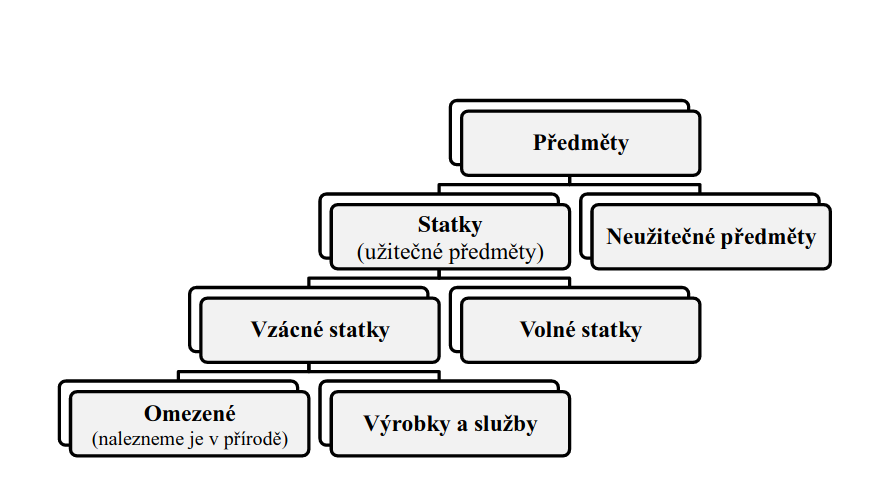
\includegraphics[width=16cm]{images/02_deleni.png}

\subsection{Výrobní faktory}
\begin{itemize}
    \item Práce (lidská činnost, přírodní zdroje -> užitečné statky, za to mzda)
    \item Půda (produkt přírody, není volný statek, i přírodní zdroje, např. nerosty)
    \item Kapitál (výsledek předchozí činnosti, hmotný nebo nehmotný, výsledkem jeho užití je zisk nebo úrok)
    \item Výrobní faktory jsou ve vlastnictví domácností a ty je pronajímají firmám za důchod. Za ten pak
    nakupují od firem statky.
\end{itemize}

\subsection{Hranice produkčních možností}
\begin{itemize}
    \item Je to křivka znázorňující různé kombinace statků nebo služeb, které mohou být vyrobeny s fixním množstvím výrobních faktorů při jejich efektivním využití.
    \item body na křivce znázorňují efektivní kombinace, body pod ní neefektivní, body nad ní nedosažitelné
\end{itemize}
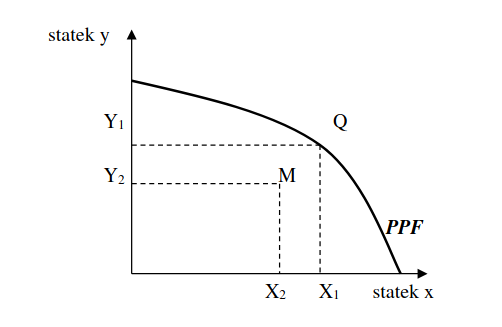
\includegraphics[width=16cm]{images/02_hranice_vyrobnich_moznosti.png}